\subsubsection{Test \ref{test15}, \enquote{Breadth First Search} button correctly shows a BFS traversal for a cyclic graph.}
Input:  7 Vertices created, A, B, C, D, E, F, G.  Edge lines exist between (A, B), (A, G), (B, C), (C, D), (D, E), (D, F), and (F, G). Click on the \enquote{Breadth First Search} button, observe the message in the status bar.
\newline
\newline
Expected output: The status bar should display \enquote{DFS: A, B, G, C, F, D, E}
\begin{figure}[ht]
    \centering
    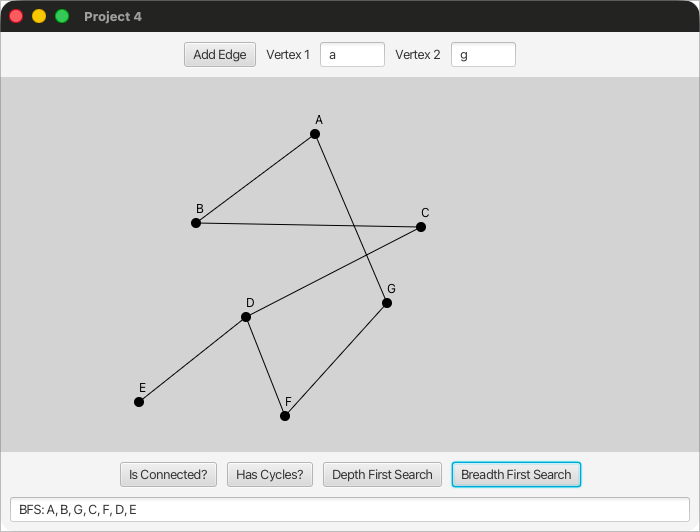
\includegraphics[width=0.65\textwidth]{images/test15.png}
    \caption{test \ref{test15}}
\end{figure}
